\section{Nedunchezhiyan K mm20b043}
\subsection{Coloumbs Law}
Coulomb force~\cite{bibfile} is the force between two stationary electric charge particle
.The equation of coulumb force is given by:
\begin{equation}
F=\frac{1}{4\pi \epsilon_0}\frac{q_1 q_2}{r^2}
\label{eqn:coloumb}
\end{equation}
\subsubsection{Terms used in the equation}
\begin{enumerate}
 \item F-viscous forece
 \item$\epsilon$-constant
 \item$\frac{q_1 q_2}{r^2}$-product of magnitude of two charges divided by square of distance between two charges
\end{enumerate}
\begin{figure}[h]
 \begin{center}
    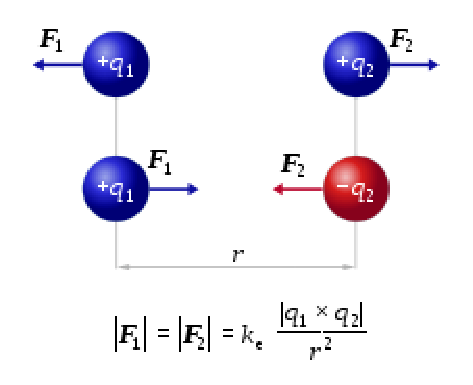
\includegraphics[scale=0.6]{mm20b043.eps}
 \end{center}
\caption{coulomb force between electric charges}
\label{fig:coloumb}
\end{figure}
\subsubsection{Description}
coulomb force obtained by using the equation~\ref{eqn:coloumb} above helps us to find force between two electrically charged particles which is essential in development of theory of electromagnetism. The same is mentioned in Figure~\ref{fig:coloumb}.
